We considered an alternative approach for setting the upper limits on
aTGC using the $CL_{s}$ method. Due to complexity of the method we had
to rely on existing tools in the Higgs group. In order to minimize
amount of work needed, we adopted a binned-likelihood appoach that may
lead to slightly different results.

The likelihood function is defined as:
\begin{eqnarray}
  L(\rm{data}|\mu,\theta)&=&\rm{Poisson}(\rm{data}|\mu\cdot s(\theta)+b(\theta))\cdot p(\tilde{\theta}|\theta) \nonumber\\
 &=&\prod_i\frac{(\mu s_i+b_i)^{n_i}}{n_i!}e^{-\mu s_i-b_i}\cdot p(\tilde{\theta}|\theta)
\label{eq:likelihood}
\end{eqnarray}
where $\mu$ is the signal strength modifier which is often reported in
the upper limit results as a ratio of the cross-section upper limit
over the standard model cross-section and $\theta$ represents a full
set of nuisance parameters that are used to incorporate systematic
uncertainties. 

As it was described earlier, the model used to parameterize aTGC
provides the leading lepton \pt\ distribution of the \ww\ system as a
function of the anomalous couplings. To extract CLs limits we had to
explicitely separate the Standard Model and anomalous parts of the
distribution. The effect of anomalous couplings on the leading
lepton \pt\ can lead to lower differential cross-section at low \pt\
values. In these cases we set the expected cross-section to be
zero. This should not have significant impact on results, since aTGC
mostly enter as events with \pt{}.

For $CL_{s}$ method the test statistic is defined as a likelihood
ratio:
\begin{equation}
\tilde{q_\mu}=-2\log\frac{L(\rm{data}|\mu,\hat\theta_\mu)}{L(\rm{data}|\hat\mu,\hat\theta)}
\end{equation}
where the numerator corresponds to the maximum likelihood for given
``data'' and $\mu$ profiling over the nuisance parameters and the
denominator corresponds to the maximum likelihood for given ``data''
profiling over the nuisance parameters and $\mu$. This test statistic
differs from the ones used at LEP (no profiling of systematic errors)
and at Tevatron (the denominator likelihood uses $\mu=0$ and only
systematic errors are profiled).

Figure~\ref{fig:cls} show the upper limit for one
and two dimentional models. The limits are found to be:
\begin{align}
  \lambda_{Z}: [-0.05,0.046]~95\%~\mathrm{C.L.}\\ 
  \Delta g^{Z}_1: [-0.084,0.07]~95\%~\mathrm{C.L.}\\
\end{align}
The results are consistent with the profiled-likelihood method. It is
important to take into account that we used the asymptotic $CL_{s}$
method, which relies on the linear behaviour of the likelihood to get
the expected limits correctly. It was found that limits extracted in
the profiled-likelihood method using explicit scan of the likelihood
(Minos) were different (smaller) than those derived using an
extrapolation (Migrad/Hesse). Producing ``full'' $CL_{s}$ limits would
take a lot of time and it is not justified for a cross-check. Without
such test the coverage of the $1\sigma$ and $2\sigma$ bands is not
guaranteed.

\begin{figure}[!hbtp]
\centering
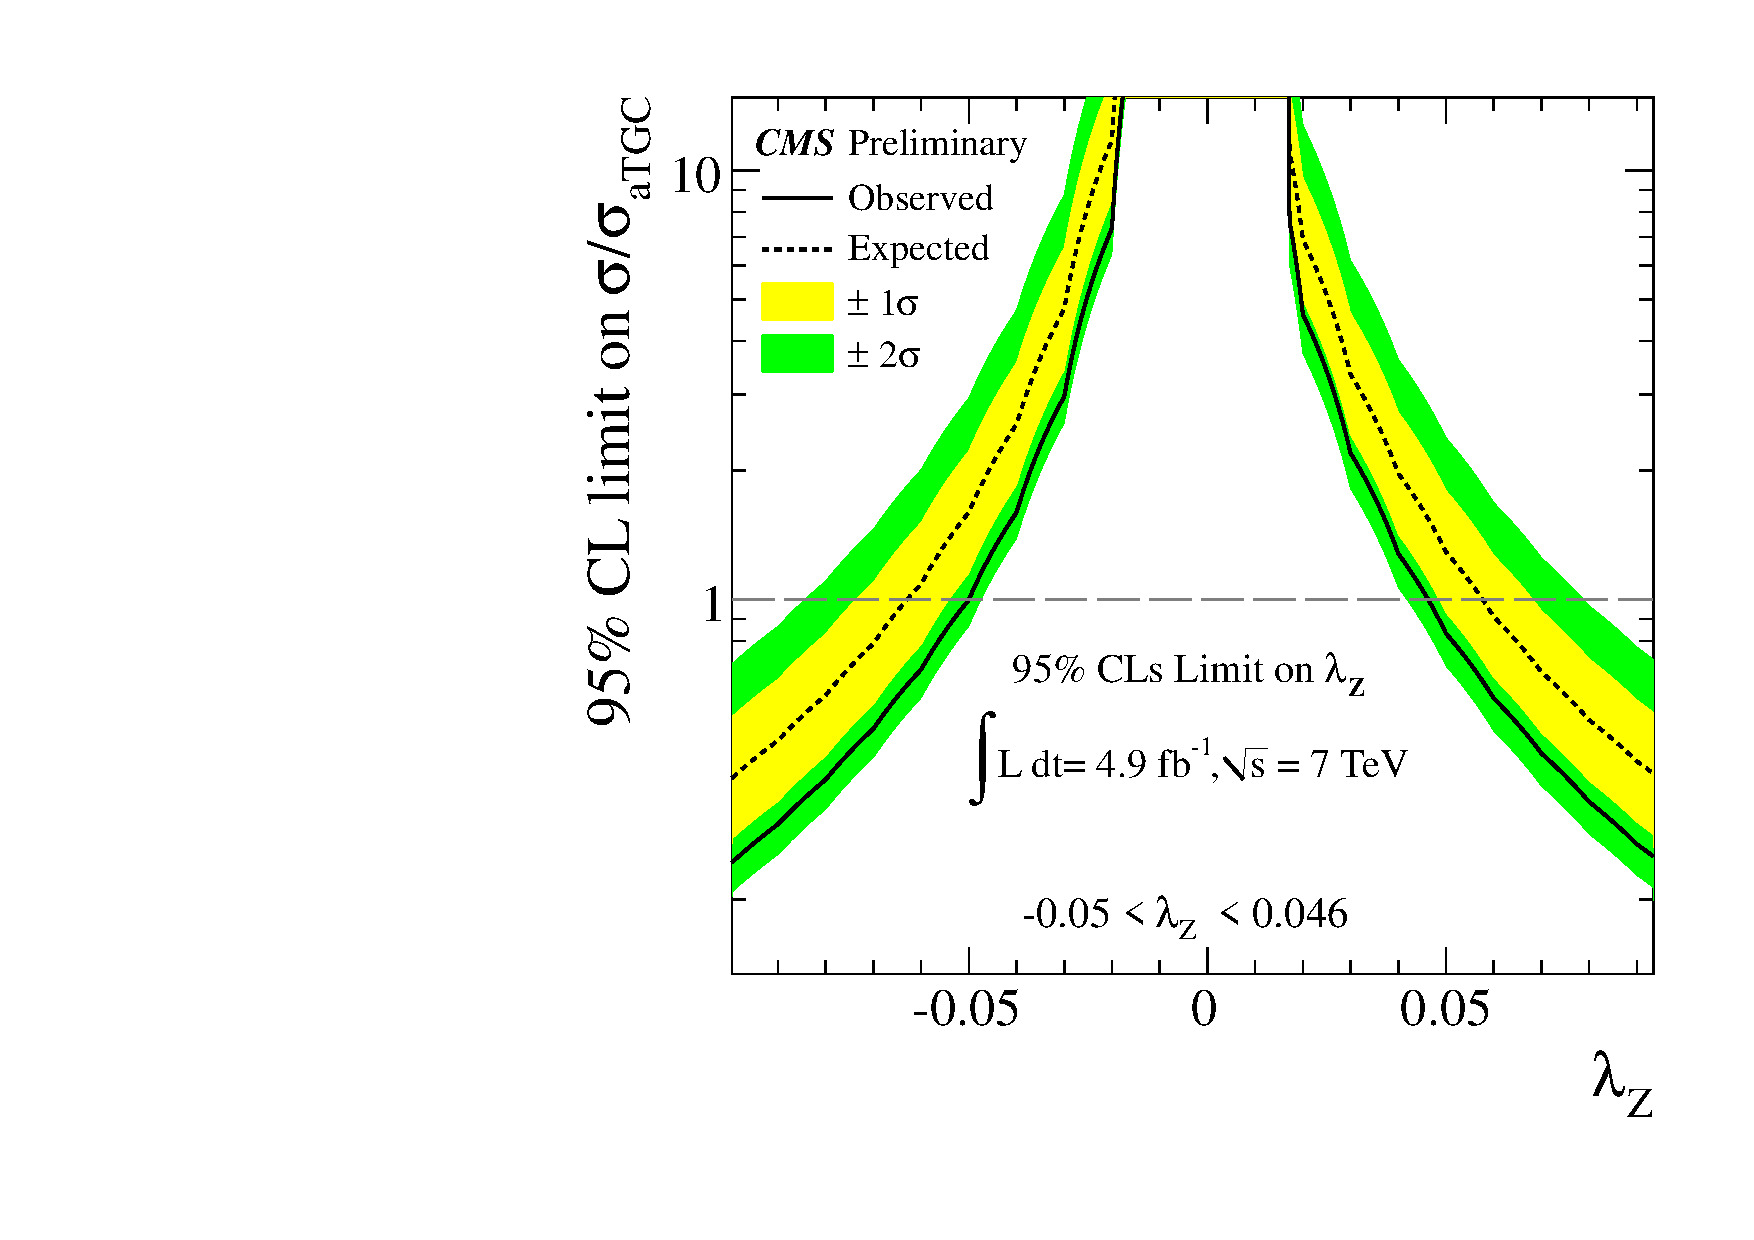
\includegraphics[width=.45\textwidth]{figures/lz_cls.pdf}
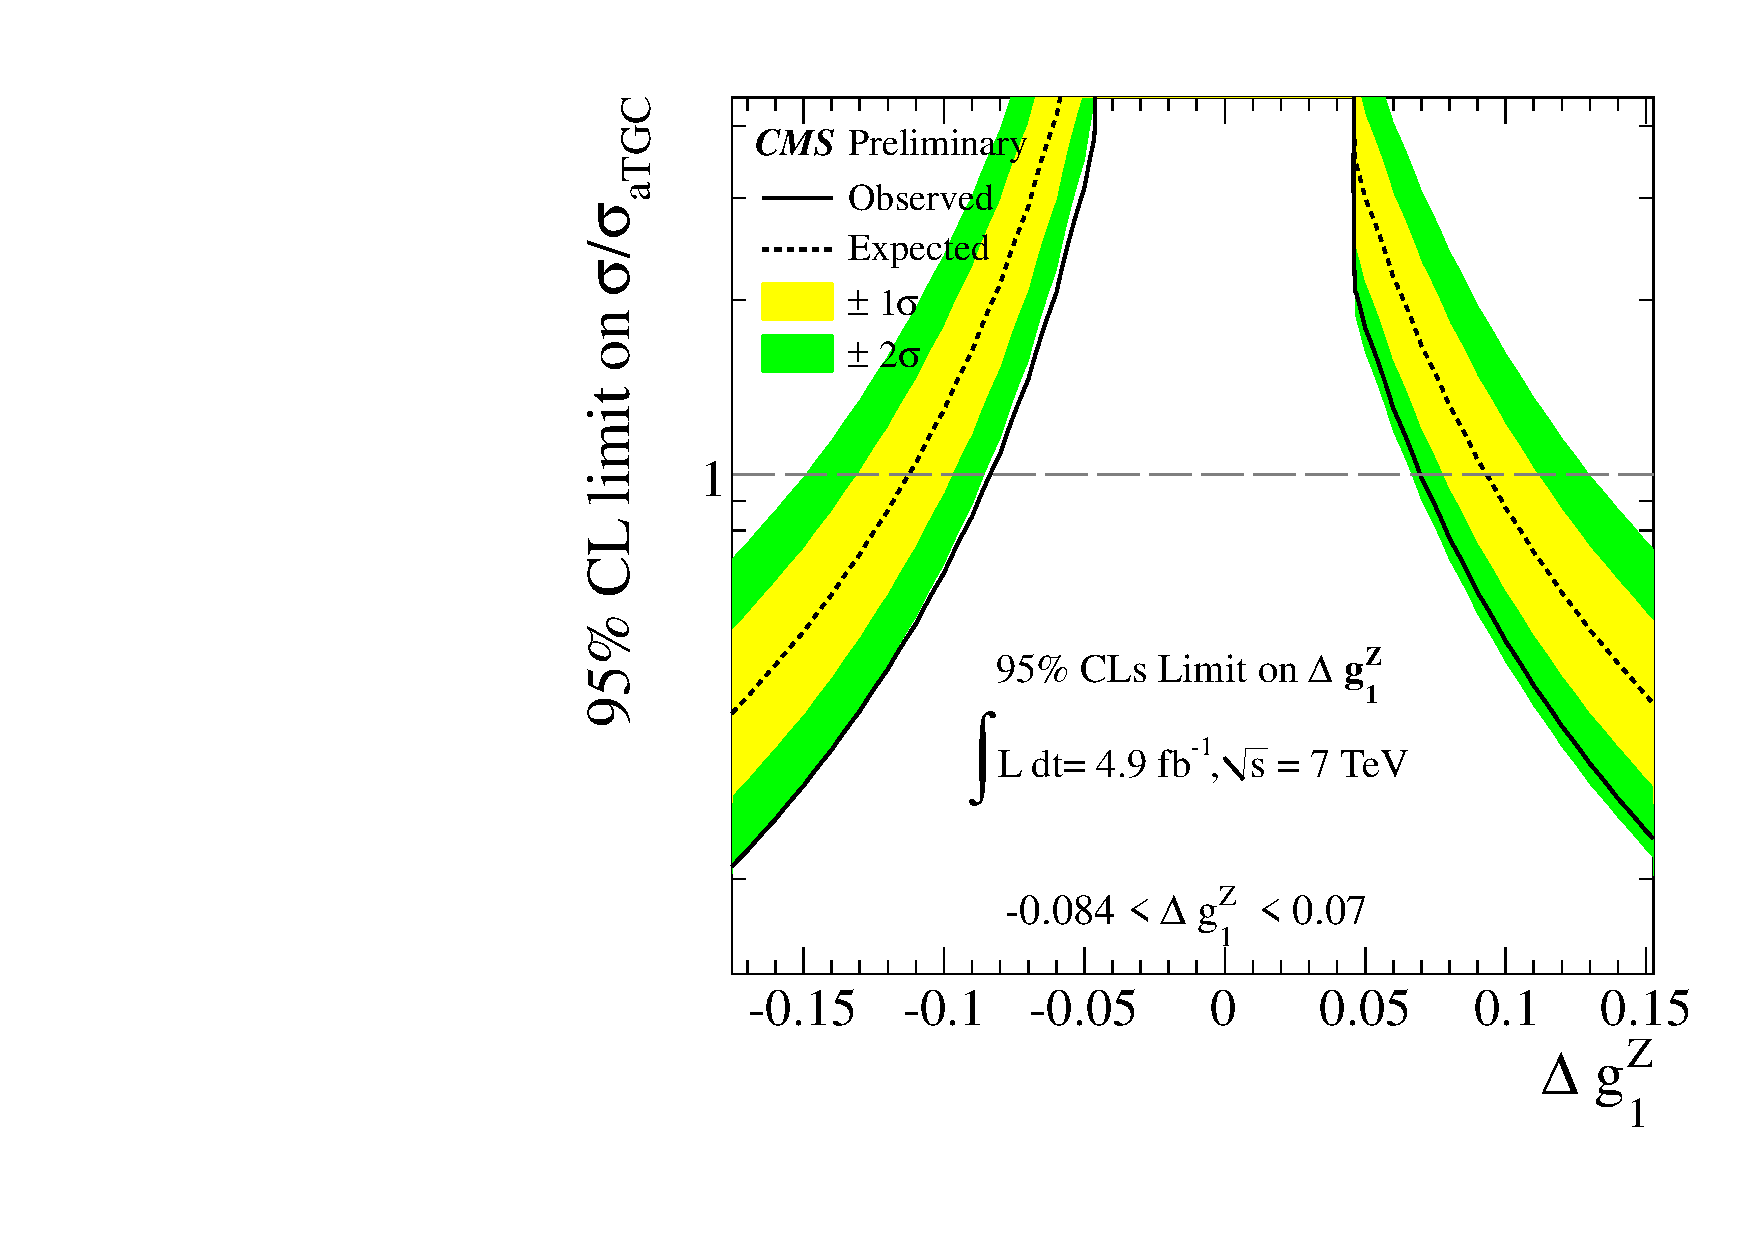
\includegraphics[width=.45\textwidth]{figures/dgz_cls.pdf}
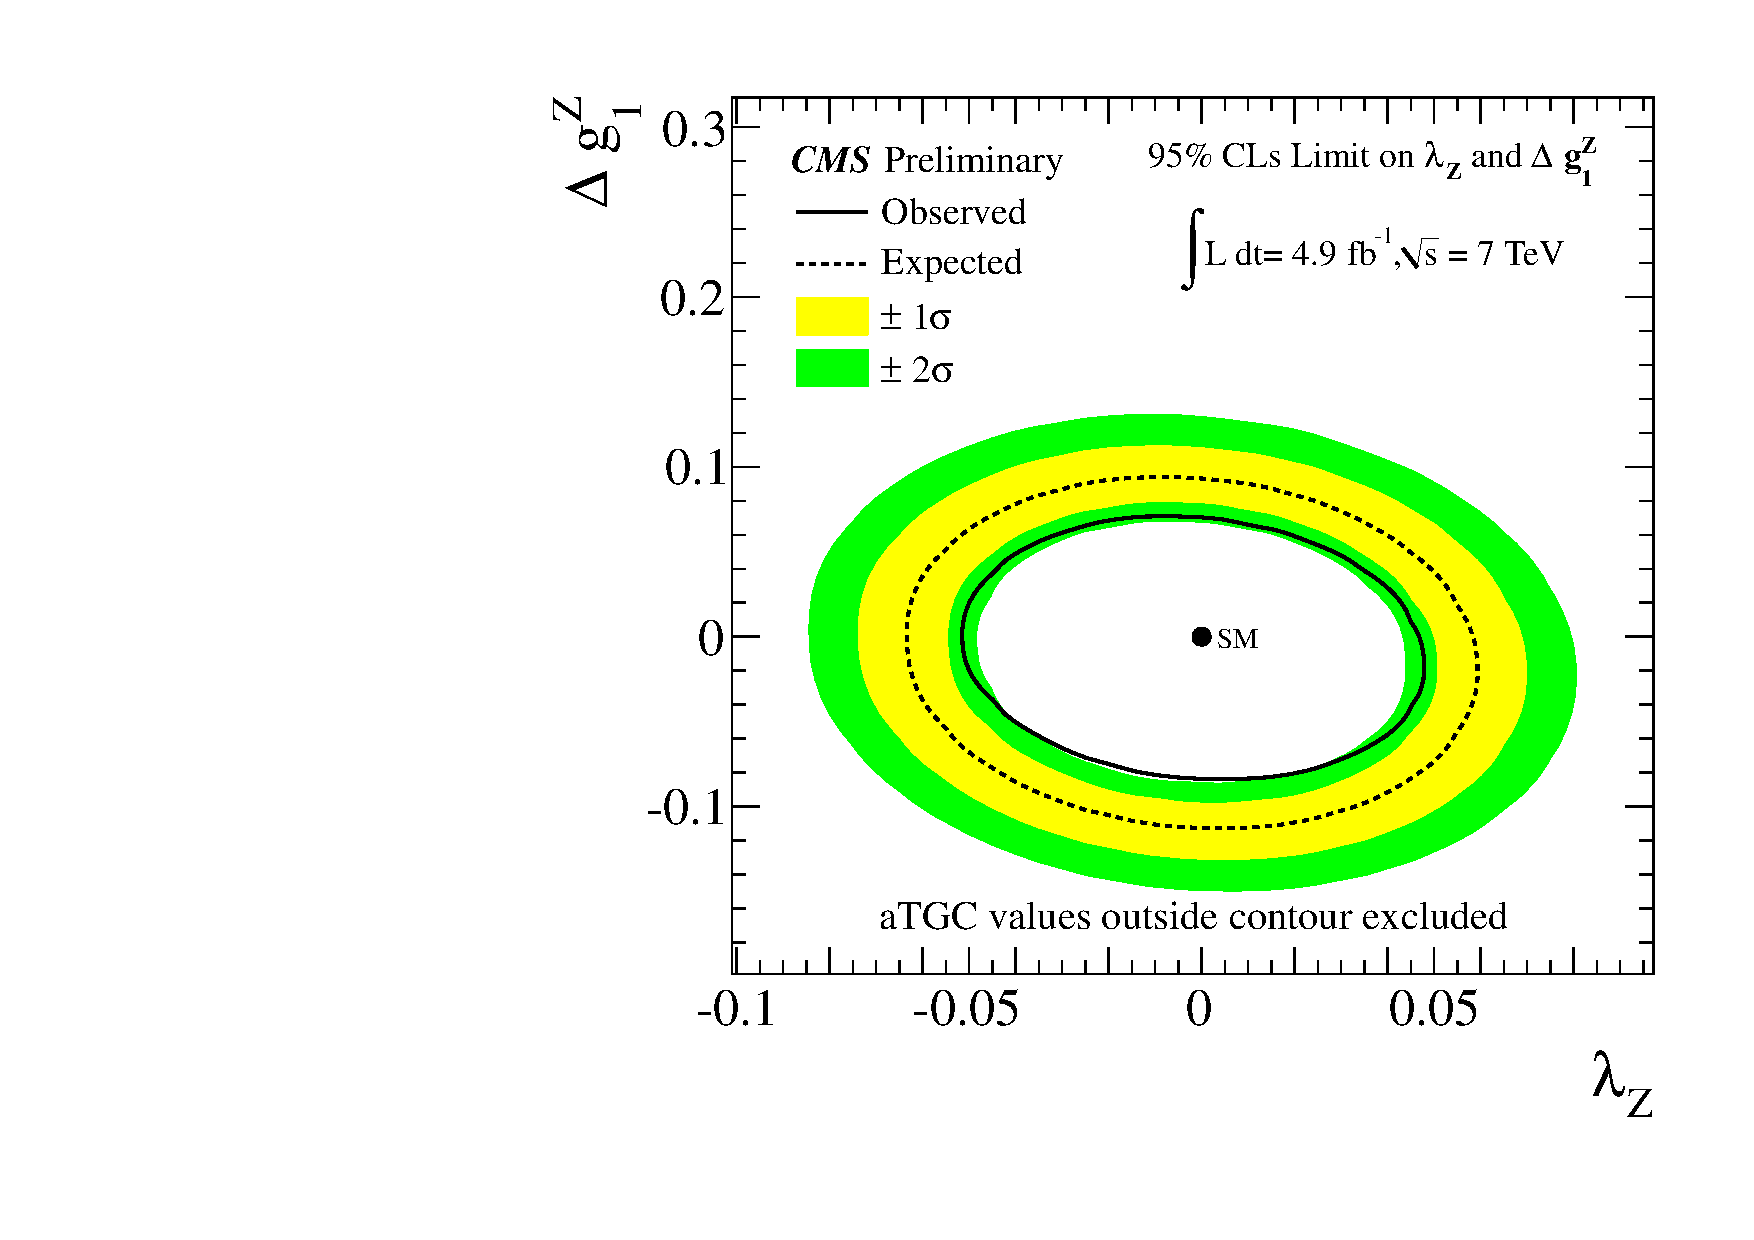
\includegraphics[width=.45\textwidth]{figures/lz_dgz_cls.pdf}
\caption{One and two dimensional $CL_{s}$ upper limits.}
\label{fig:cls}
\end{figure}
